
\begin{frame}{Markov Decision Process(MDP)}{Qu'est ce que la décision de Markov}
	\begin{center}
		\begin{block}{Objectif}
			Lorsque le modèle rencontre un problème, il existe plusieurs manières de le résoudre. On cherche la meilleure solution. Lorsque l'on répète cette action, on appelle cela un processus de décision de Markov. 
		\end{block}
		\begin{block}{Principe}
			Un agent est capable de comprendre l’état dans lequel se trouve son environnement, et doit être en mesure de trouver une réponse afin de le modifier si besoin.
		\end{block}
	\end{center}
\end{frame}
\begin{frame}{Markov Decision Process(MDP)}{Fonctionnement de l'apprentissage par renforcement}
	\begin{center}
		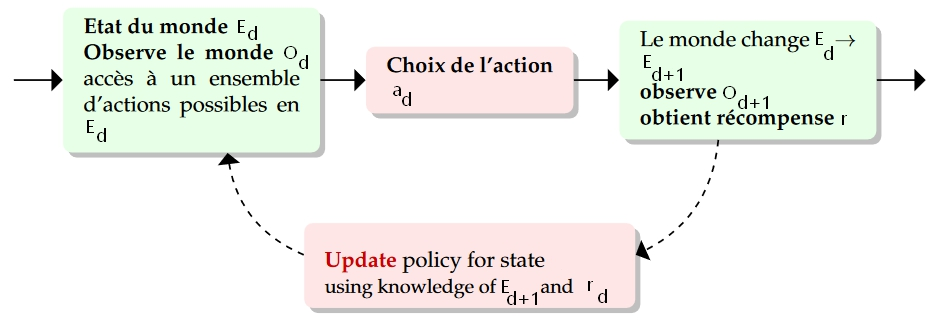
\includegraphics[width=10cm]{ressources/MDP/Fonctionnement.jpg}
	\end{center}
	\begin{block}{Objectif}
		Maximiser les récompenses.
	\end{block}
\end{frame}
\begin{frame}{Markov Decision Process(MDP)}{Qu'est ce qu'un état de Markov ?}
	\begin{center}
		
		\begin{block}{Visualisation}
			L'environnement est visualisable comme un automate probabilisé.
		\end{block}
		\begin{block}{Etat}
			On peut noter la probabilité d'arriver dans un état comme cela:\\
			Notons $E_{i}$ tous les états. Pour $i \in [1,d]$ avec $d$ l'indice du dernier état connu.\\
			Alors un état $E_{d+1}$ est dit de Markov si et seulement si :\\ 
			$$\mathbb{P}(E_{d+1} | E_{d}) = \mathbb{P}(E_{d+1} | E_{1}, ..., E_{d})$$\\
		\end{block}
		\begin{block}{Avantage}
			Ainsi l'état suivant ne dépend pas de tous les évènements qui ont précédés, mais juste de l'état précédent, comme aux échecs.
		\end{block}
	\end{center}
\end{frame}
\begin{frame}{Markov Decision Process(MDP)}{Maximiser les récompenses}
	\begin{center}
		
		\begin{block}{Fonction de récompense}
            \centering
			$R_t = \sum^{\infty}_{k=0}\gamma^{k}r_{t+k+1}$
		\end{block}
		\begin{block}{Explications}
			$r_{i}$ est la récompense obtenue au $i$-ième état.
			$\gamma$ est appelé facteur de dévaluation.\\
			$\gamma$ = 0 : l'agent ne voit rien, il ne veut que des récompenses immédiates.
			$0< \gamma <1$ cherche un équilibre entre la récompense immédiate et celles futures.
		\end{block}
		\begin{block}{Comment choisir le prochain état ?}
			La fonction valeur évalue la qualité d’un état, et ou d’une action. En se basant sur l’espérance du gain possible atteignable directement, et des gains qui pourront en découler. Ainsi elle permet de choisir l’action la plus favorable.
		\end{block}
	\end{center}
\end{frame}
\begin{frame}{Markov Decision Process(MDP)}{Chaines de Markov}
	\begin{center}
		
		\begin{center}{Un exemple d'automate}
			\includegraphics[width=9.8cm]{ressources/MDP/automate probabilisé.png}
		\end{center}
	\end{center}
\end{frame}
\begin{frame}{Markov Decision Process(MDP)}{Sous forme de matrice}
	\begin{center}
		\begin{center}{Matrices de transition}
			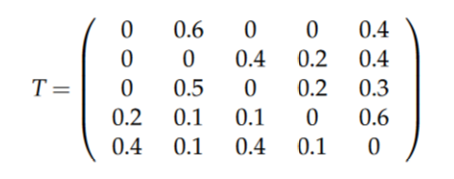
\includegraphics[width=10cm]{ressources/MDP/Matrice de transitions.png}
		\end{center}
	\end{center}
\end{frame}
\begin{frame}{Markov Decision Process(MDP)}{}
	\begin{center}
		\begin{block}{Markov Decision Process}
			Un Markov Decision Process est un tuple $<E,A,T,R,\gamma>$ où :\\
			$E$ est un ensemble fini d'états.\\
			$A$ est un ensemble fini d'actions.\\
			$T$ est une matrice de transition.\\
			$R$ sont les récompenses.\\
			$\gamma$ est le facteur de dévaluation.
		\end{block}
	\end{center}
\end{frame}
